\section{Limiting Factors of the GPU}

In order to write code that is accelerated by the GPU, we must know which factors impact performance and to what extend. 
For this we have measured the performance of the following metrics: 

\begin{itemize}
    \item Allocating and freeing memory on the GPU
    \item Copying memory to and from the GPU
    \item Spawning more blocks for a single kernel.
\end{itemize}

To measure these metrics, we have used our automated benchmarking tool. Each algorithm was run with an exponentially scaling input to see how the performance of the operation scales. The code being measured can be seen below.

\begin{lstlisting}[language=C, caption={Code to measure allocating and freeing memory}, label={lst:cudaMalloc}]
void malloc_scaling_with_dimension(matrix_t *matrix) {
    device_matrix_t device_matrix =
        cuda_matrix_init(matrix->rows, matrix->columns);
    cuda_matrix_free(device_matrix);
}
\end{lstlisting}


\begin{lstlisting}[language=C, caption={Code to measure moving memory}, label={lst:cudaMemcopy}]
void memcpy_scaling_with_dimension(matrix_t *matrix) {
    device_matrix_t device_matrix =
        cuda_matrix_init(matrix->rows, matrix->columns);
    cuda_matrix_host_to_device(device_matrix, matrix);
    cuda_matrix_device_to_host(matrix, device_matrix);
    cuda_matrix_free(device_matrix);
}
\end{lstlisting}

\begin{lstlisting}[language=C, caption={Code to measure spawning more blocks}, label={lst:noop}]
__global__ void noop_kernel() {}

void launch_kernel_scaling_with_dimension(int dimension) {
    noop_kernel<<<dimension, 1024>>>();
}
\end{lstlisting}

These were our chosen points of interest to benchmark at the point in time when we had implemented matrix addition and matrix multiplication on the GPU. 
Crucially this meant we had only ever launched a single kernel to run our algorithm on the GPU and did not think to benchmarking the cost of launching kernels. 
This had major impact on the design of our QR-decomposition algorithm, which will be discussed later. 
In the end we measured two more metrics:
\begin{itemize}
    \item Launching kernels asynchronously
    \item Launching kernels synchronously
\end{itemize}

\begin{lstlisting}[language=C, caption={Code to measure the launch of asynchronous kernels}, label={lst:asynchronous kernels}]
void launch_x_kernels(int dimension) {
    for (int i = 0; i < dimension; i++)
    {
        noop_kernel<<<1, 1>>>();
    }
}
\end{lstlisting}

\begin{lstlisting}[language=C, caption={Code to measure the launch of synchronous kernels}, label={lst:synchronous kernels}]
void launch_x_kernels_sequentially(int dimension) {
    for (int i = 0; i < dimension; i++)
    {
        noop_kernel<<<1, 1>>>();
        cudaDeviceSynchronize();
    }
}
\end{lstlisting}

\subsection{Observations}

\color{red}
insert diagram of diagnostics comparrison
\color{black}

From our analysis we can conclude the following: 
The amount of blocks and threads spawned to execute a single kernel has no impact on performance. 
Allocating and freeing memory is done in constant yet significant amount of time. 
Copying memory to and from the GPU takes an insignificant amount of time, until millions of floats are being transferred. 
Launching a kernel takes a significant amount of time. 

\begin{figure}[ht]
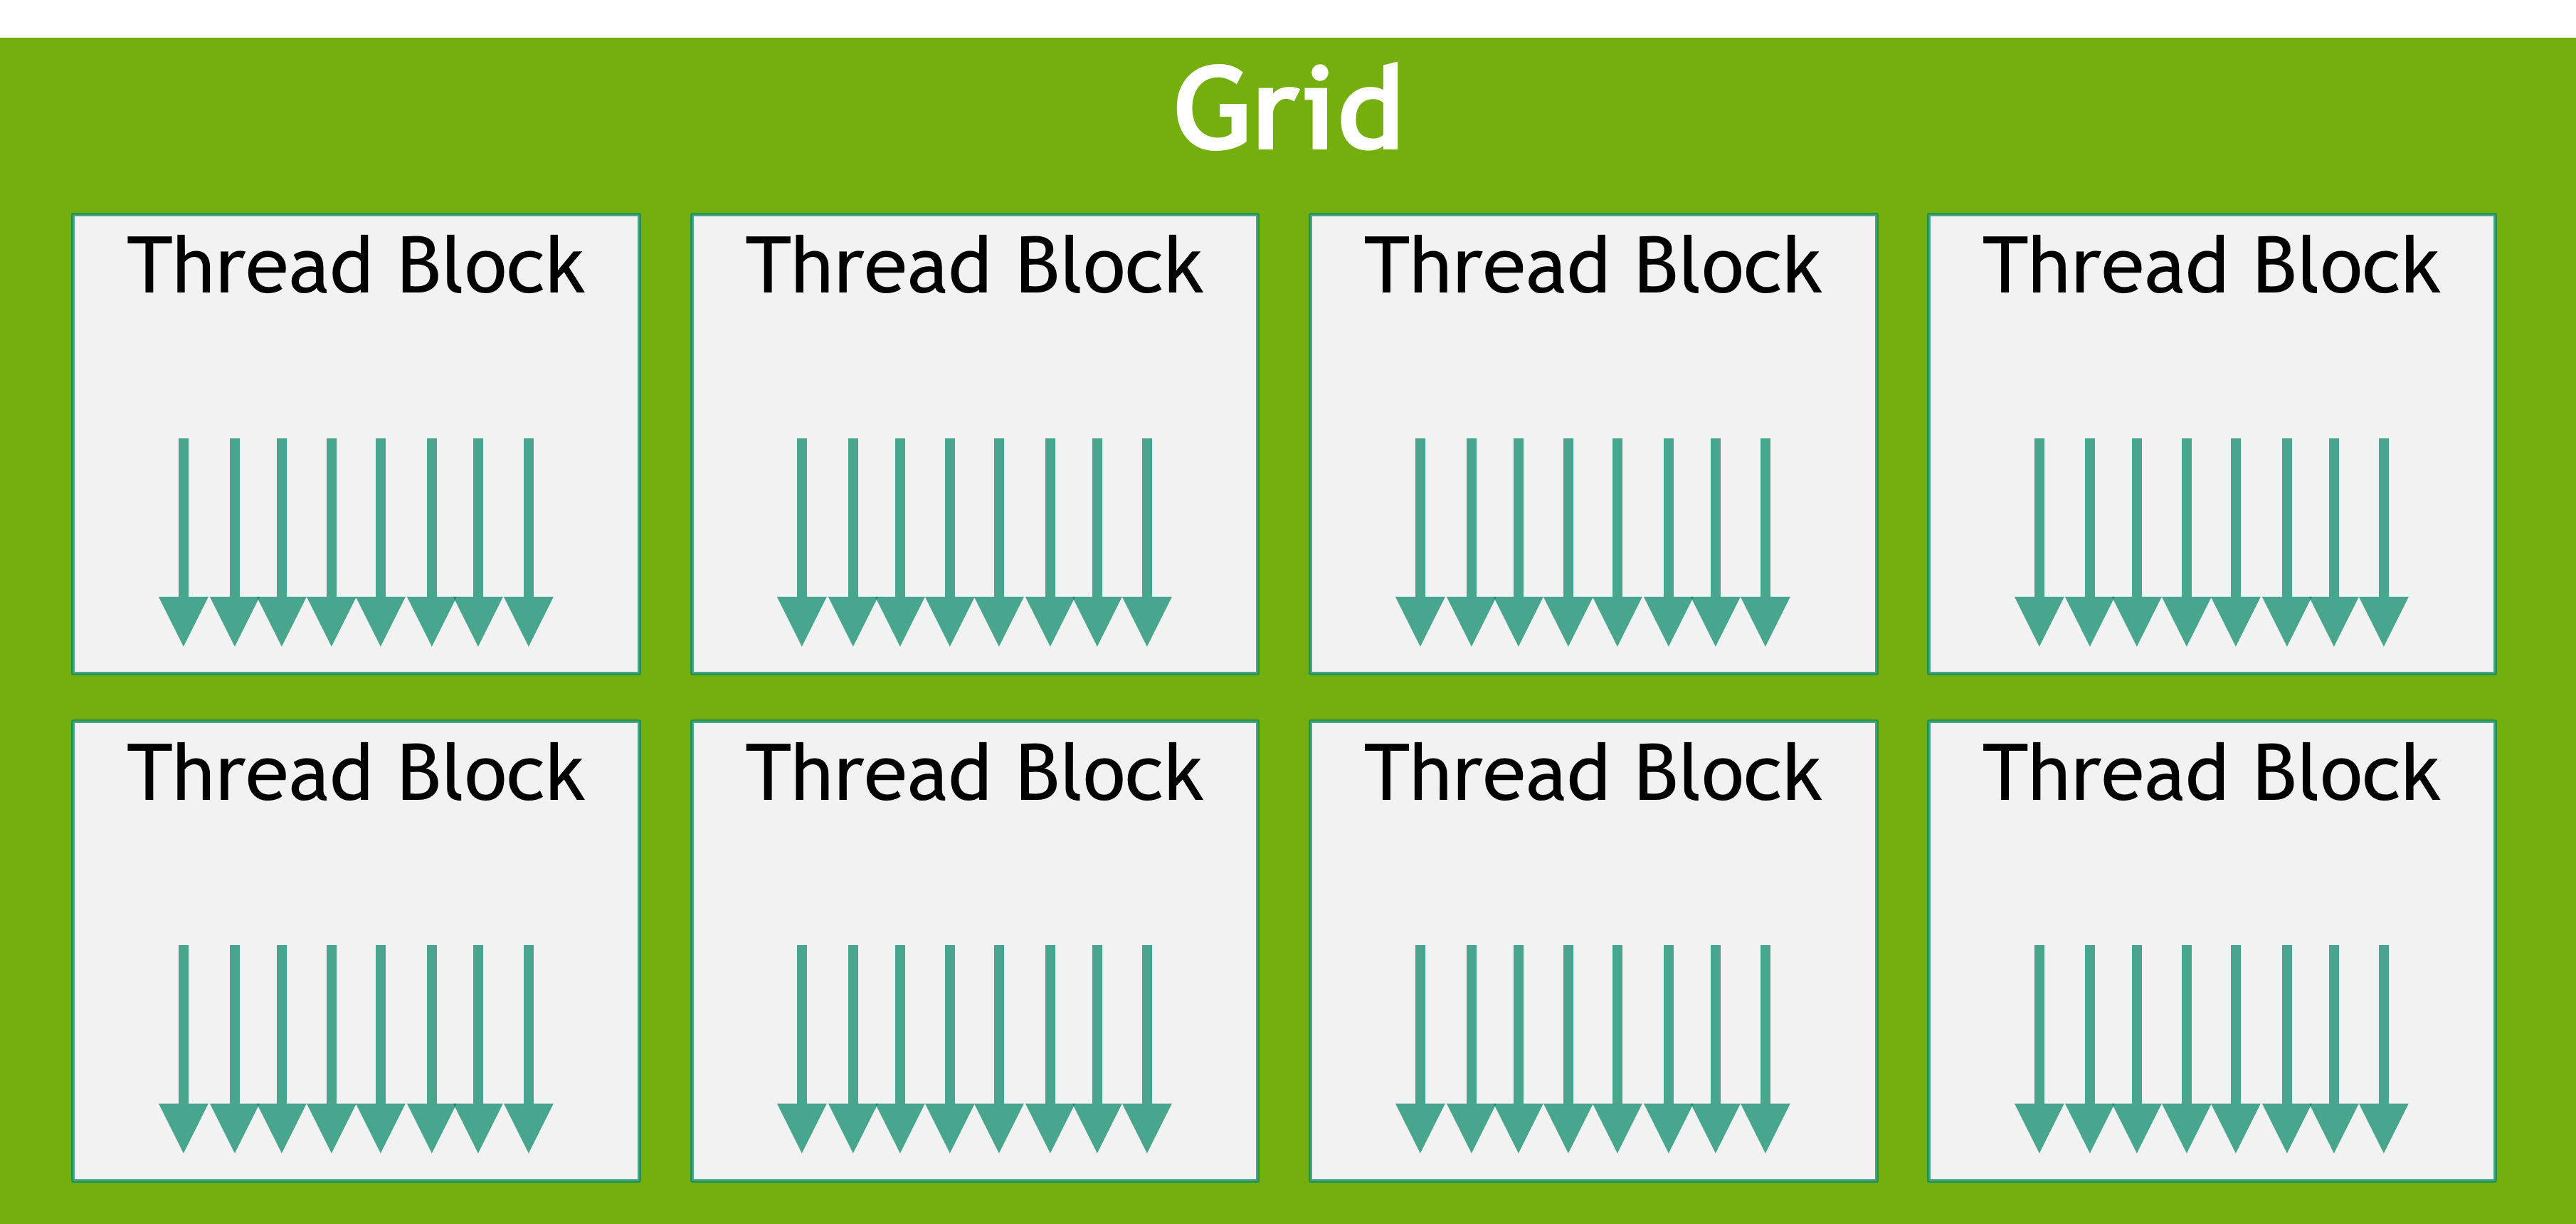
\includegraphics[width=\textwidth]{Documents/Report/Figures/Threads and blocks.png}
\caption{Threads inside thread blocks inside the grid. From \cite{nvidia:cudadoc}}
\label{fig:threads and blocks}
\end{figure}
